\section{Distribution of IP Addresses on Autonomous Systems}\label{sec:aslevel:census}

The performance of systems using CPE or resources provided by end-users depend on the capacity and number of devices available.
To assess the potential of a hierarchical cache system in an ISPs network, the number of active subscribers in an autonomous systems has to be known.
Assuming that the number of active IP-addresses is correlated to the number of subscribers in an autonomous system, we use the Internet Census Dataset to determine the distribution of active IP-addresses on autonomous systems.

The Internet Census Dataset\cite{carna2013} was conducted from June to October 2012.
The complete IPv4-address room was scanned using a bot-net consisting of 4,200,000 nodes.
In the ICMP ping scan more than 420 million replied to requests more than once.
The service probe data reveal open ports on devices which is used to infer the type of device.
The Internet Census Dataset was validated forensically in \cite{dainotticaida}.
In \cite{krenc2014internet} the scope of the dataset is taken into perspective and show that, although there are some qualitative problems, the measurement data seems to be authentic.
%We use the Internet Census Dataset to determine the number of active IP-addresses for each autonomous system in the Internet.

We use an IP to ASN mapping to derive the autonomous system number for each IP-address. There are different services, that provide an IP to ASN mapping.
The whois-service can be used to get the current ASN for an IP-address.
To enable an efficient evaluation we used the MAXMIND GeoLite ASN database \cite{geo_ip}, which is updated every month and can be downloaded and used as a local database.
The results of the MAXMIND GeoLite ASN database were cross checked with results obtained from whois, which showed no differences.

The ICMP ping scan discovered a total of 598,180,914 IP-addresses.
The service probe scan discovered 244,000 IP-addresses that listen to port 9100 and are identified as print servers, and 70.84 million IP-addresses of web-servers that listen to port 80.
Assuming that most network functions do not reply to ICMP ping requests and neglecting different network functions, this results in 88.1\% of IP-addresses assigned to end-user devices.
Since the Internet Census the number of Internet users increased, which also has to be considered.
According to \cite{itu2015facts} there is a 7\% annual increase in fixed-broadband subscriptions in the past three years.
%From 2012 to 2014 the number of Internet users increased by almost 500,000,000 according to \cite{•}.

% \begin{figure}[tb]
% \centering
% 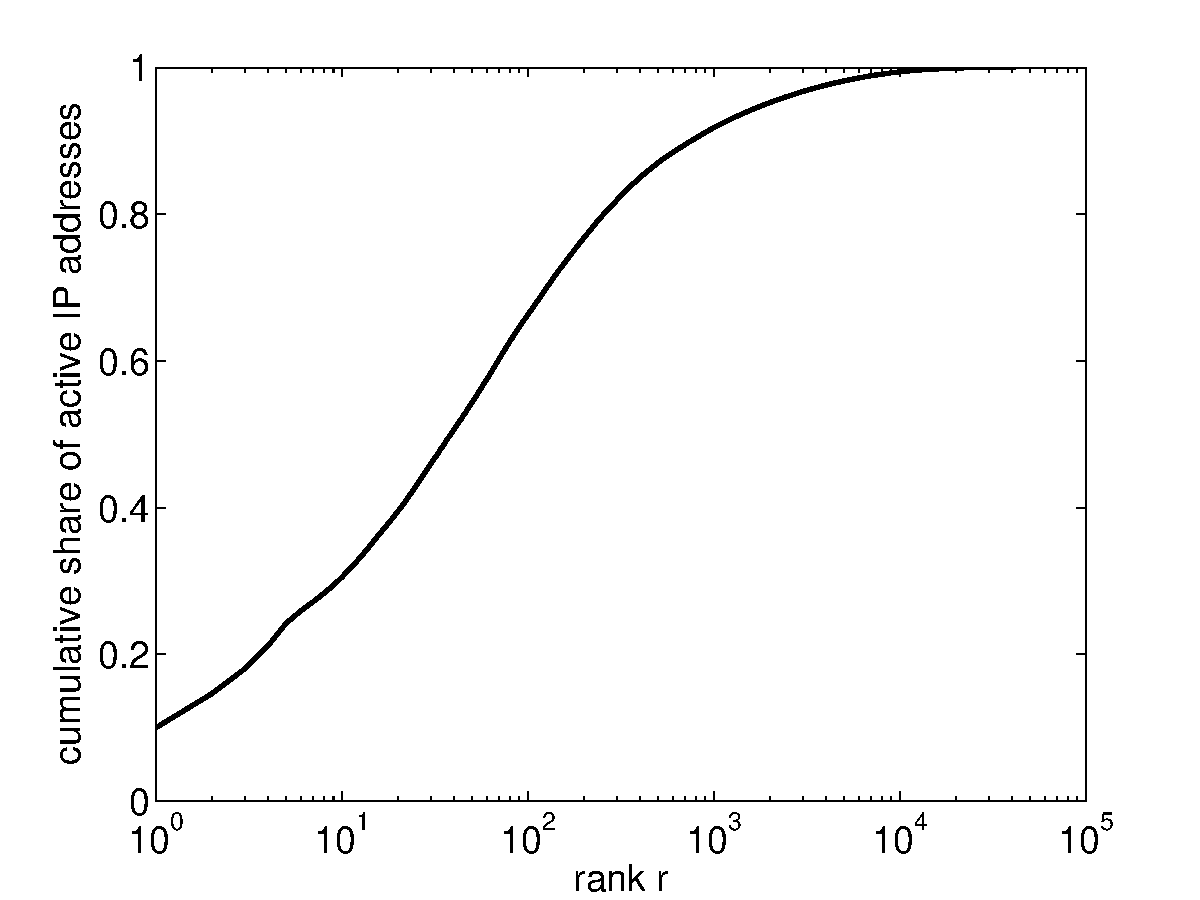
\includegraphics[width=0.49\textwidth]{aslevel/census/figs/shareactiveIPs}
% \caption{Cumulative share of active IP-addresses in autonmous systems ranked in descending order.}
% \label{fig:shareactiveIPs}
% \end{figure}
%
% \begin{figure}[tb]
% \centering
% 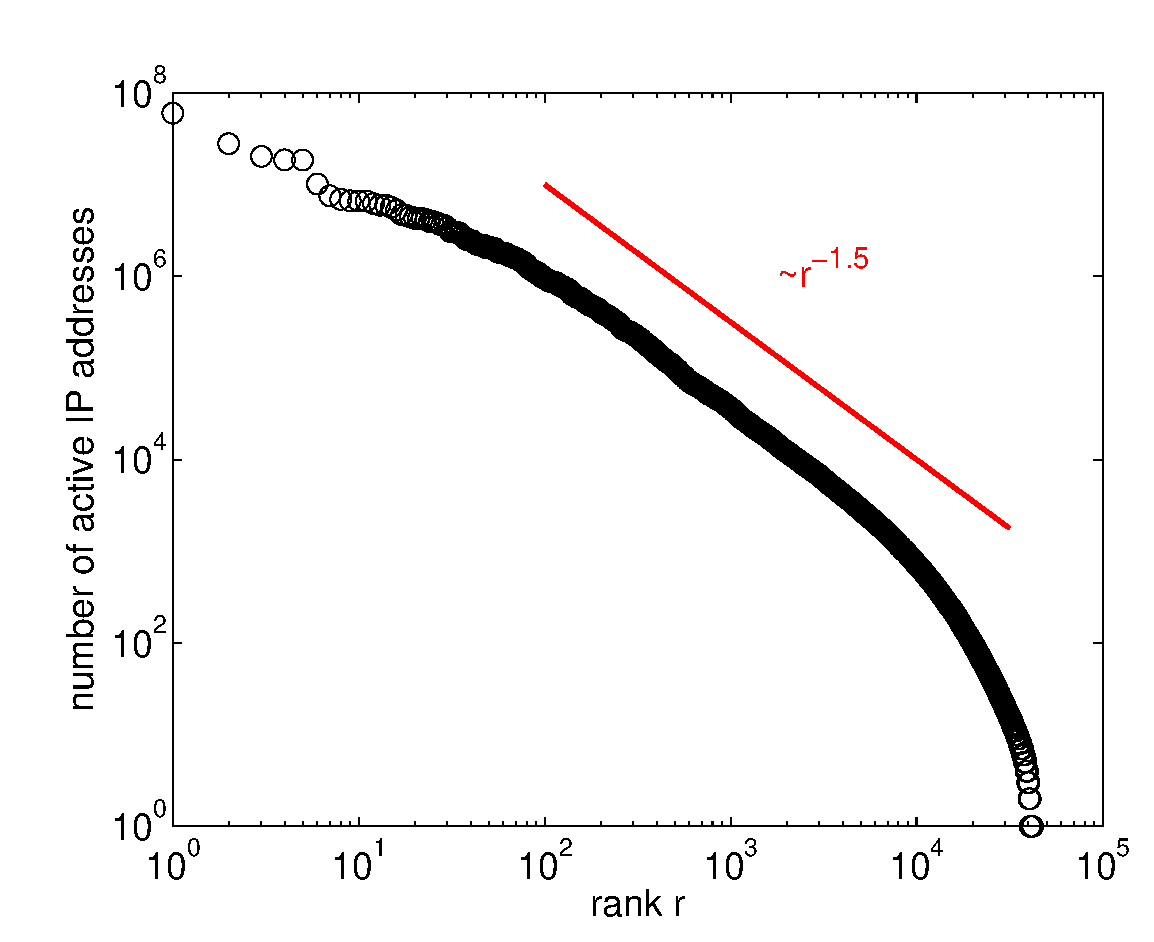
\includegraphics[width=0.49\textwidth]{aslevel/census/figs/activeIPs}
% \caption{Rank of Internet providers with number of active IP-addresses per AS.}
% \label{fig:asrank}
% \end{figure}

\begin{figure*}[bt]
\begin{minipage}[b]{0.49\textwidth}
  \centering
  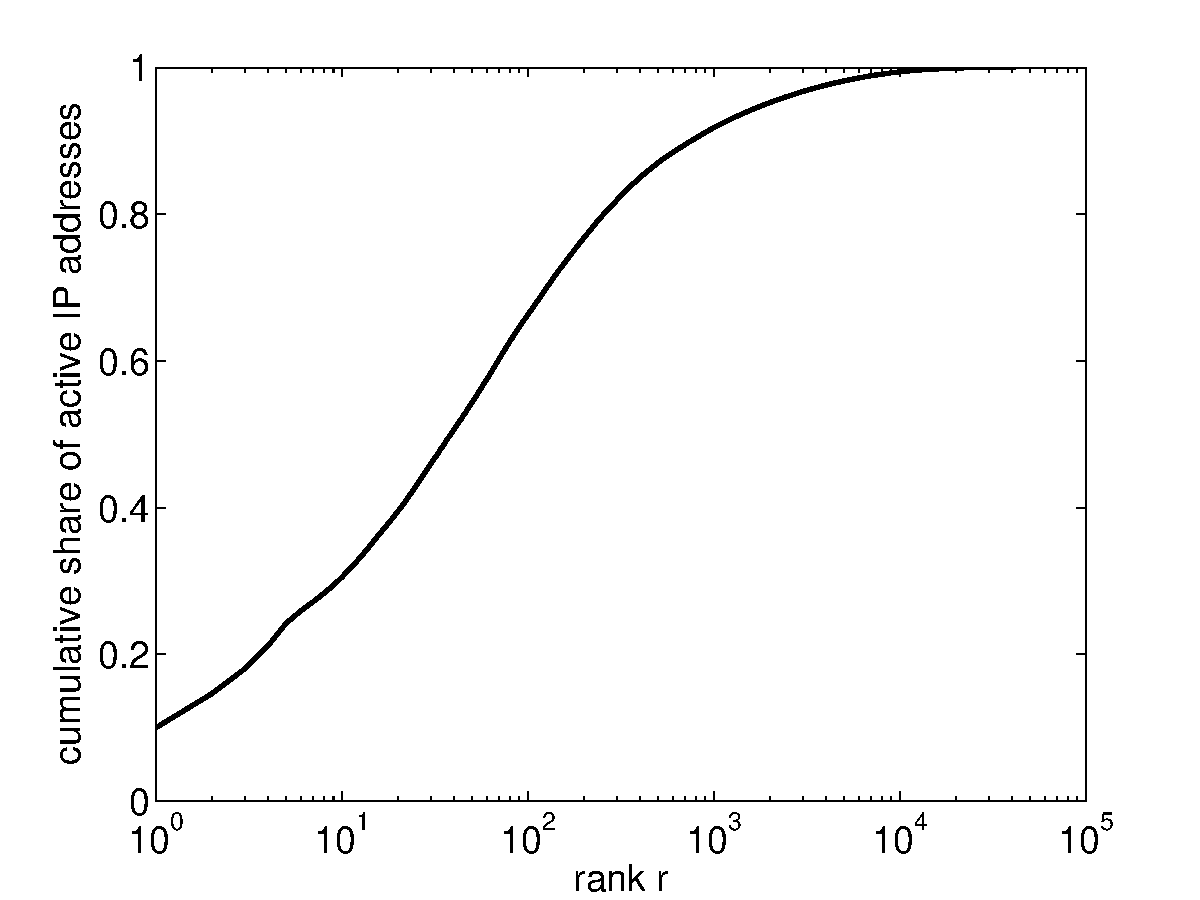
\includegraphics[width=1\textwidth]{aslevel/census/figs/shareactiveIPs}
  \caption{Cumulative share of active IPs in autonmous systems ranked in descending order.}
  \label{fig:shareactiveIPs}
\end{minipage}
\hspace{0.01\textwidth}
\begin{minipage}[b]{0.49\textwidth}
  \centering
  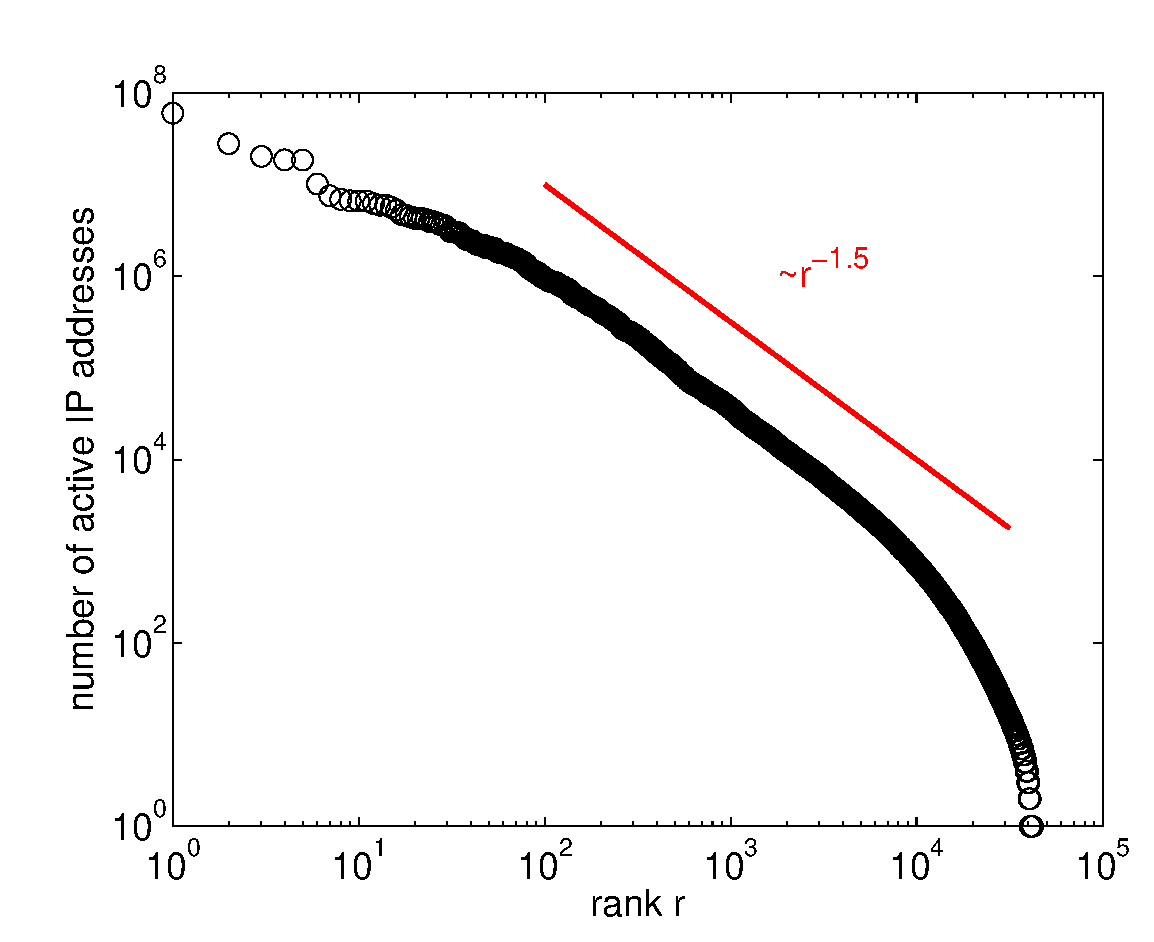
\includegraphics[width=\textwidth]{aslevel/census/figs/activeIPs}
  \caption{Rank of Internet providers with number of active IPs per AS.}
  \label{fig:asrank}
\end{minipage}
\end{figure*}

\reffig{fig:shareactiveIPs} shows the cumulative share of active IP-addresses in the autonomous systems ranked in descending order.
The 100 largest autonomous systems make up 2/3 of active IPs and more than 85\% of the IPs are active in only 1\% of the autonomous systems. The 10 largest autonomous systems already contain 30\% of the active IPs.

\reffig{fig:asrank} shows the number of active IP-addresses per AS ranked in descending order.
The top 5 ASs are shown in table~\ref{tab:asrank}.
The AS with most active IP-addresses is ChinaTelecom with almost 60 million active IPs, followed by another Chinese provider.
The largest AS in the US is Comcast on rank three.
The largest Korean and German providers are ranked 4 and 5 with more than 18 million active IPs.
The number of active IP addresses can be approximated with a power law with slope 1.5 that drops a little for low ranks.
This shows that the distribution of active IP addresses on ASs is highly heterogeneous.
That means the potential of approaches leveraging spare resources on home gateways depends on the AS.

\begin{table}[tb]
\centering
\caption{Rank of top 5 provider with most active IP-addresses.}
\label{tab:asrank}
\begin{tabular}{|c|c|c|c|}
\hline
rank r & ASN & provider & \# active IPs  \\
\hline
1 & 4134 & ChinaTelecom & 59,824,824 \\
2 & 4837 & China-Network-Communication-Group & 27,776,643 \\
3 & 7922 & Comcast & 20,227,918 \\
4 & 4766 & KoreaTelecom & 18,502,963 \\
5 & 3320 & DeutscheTelekomAG & 18,476,519 \\
\hline
\end{tabular}
\end{table}
%

%\input{aslevel/census/dataset/dataset}
%\subsection{Numerical Examples and Impact on Transit Costs}\label{sec:hierarchical:simulative:evaluation}

To evaluate the performance of a CDN supported by home routers, two scenarios are simulated. The first scenario simulates requests to a CDN with caches organized in a tree structure and compares isolated caches to cooperating caches to assess the benefit of the overlay.
The second scenario adds an AS topology with peering and transit links to evaluate the inter-domain traffic saving potential.
As described in \refchap{chap:aslevel} a transit link exists between a customer ISP and its transit provider, if the customer ISP pays the transit provider to forward its traffic destined to parts of the Internet that the customer ISP does not own or cannot reach.

%\subsection{Caching}
% To assess the impact of the number of shared home routers and the size of the ISP, a tiered caching architecture with resource locations at three different tiers, including the main data center of the content provider, CDN caches, and end-user equipment is evaluated.
% The number of different content items to be downloaded or streamed from the resources is specified by the catalog size $N$. Tier-3 resource is the data center of the content provider, where all $N$ content items are stored. Tier-2 resources are edge caches and ISP caches, typically organized in a CDN, which are located close to Internet exchange points or within ISP networks. Requests served by ISPs or edge caches produce less or no inter-domain costs. Thus, these caches are referred as ISP caches in the following. The capacity of ISP caches is given as a fraction of $N$ and is specified by $C_{ISP}$. The caching strategy of ISP caches is LRU.
%Each autonomous system hosts an ISP cache.
Within tier-1, the caches are placed on shared home routers. These caches are referred to in the following as home routers (HRs). The cache capacity of HRs is specified by $C_{HR}$ and their caching strategy is LRU. In this study $C_{HR}$ is set to four (4) content items.
We evaluate the performance dependent on the autonomous system size $n_\text{user}$, in terms of the number of end-users in the autonomous system. The probability that an end-user enables the HR to shares contents is given by $p_\text{share}$. The probability that a user requests certain content items depends on the content's popularity distribution, which is specified by the Zipf exponent $\alpha$.

\subsubsection{Benefits of an Overlay}

To evaluate the performance of the overlay, two cases are considered (a) the tree case and (b) the overlay case. In the tree case (a), each user is assigned to one shared HR in its AS. If a user shares its HR, it is assigned only to its HR. A requested item is looked up in the assigned HR initially, i.e. in the tier-3 cache. If the requested item is not found, the request is forwarded to the next tier. The hierarchic caching strategy is leave-copy-everywhere, which means that the video is cached in each cache on the look up path. In the overlay case (b), a requested item is looked up in the HR of the user, if it is not found, it is looked up in shared HRs in the same autonomous system using the overlay. If no tier-3 cache in the AS contains the item it is looked up in tier-2 caches and finally in the data center of the content provider. The hierarchic caching strategy is leave-copy-everywhere, too, with the constraint, that the item is cached in the tier-3 cache only, which was looked up first.

\begin{figure*}[tb]
\centering
\begin{subfigure}[t]{0.32\textwidth}
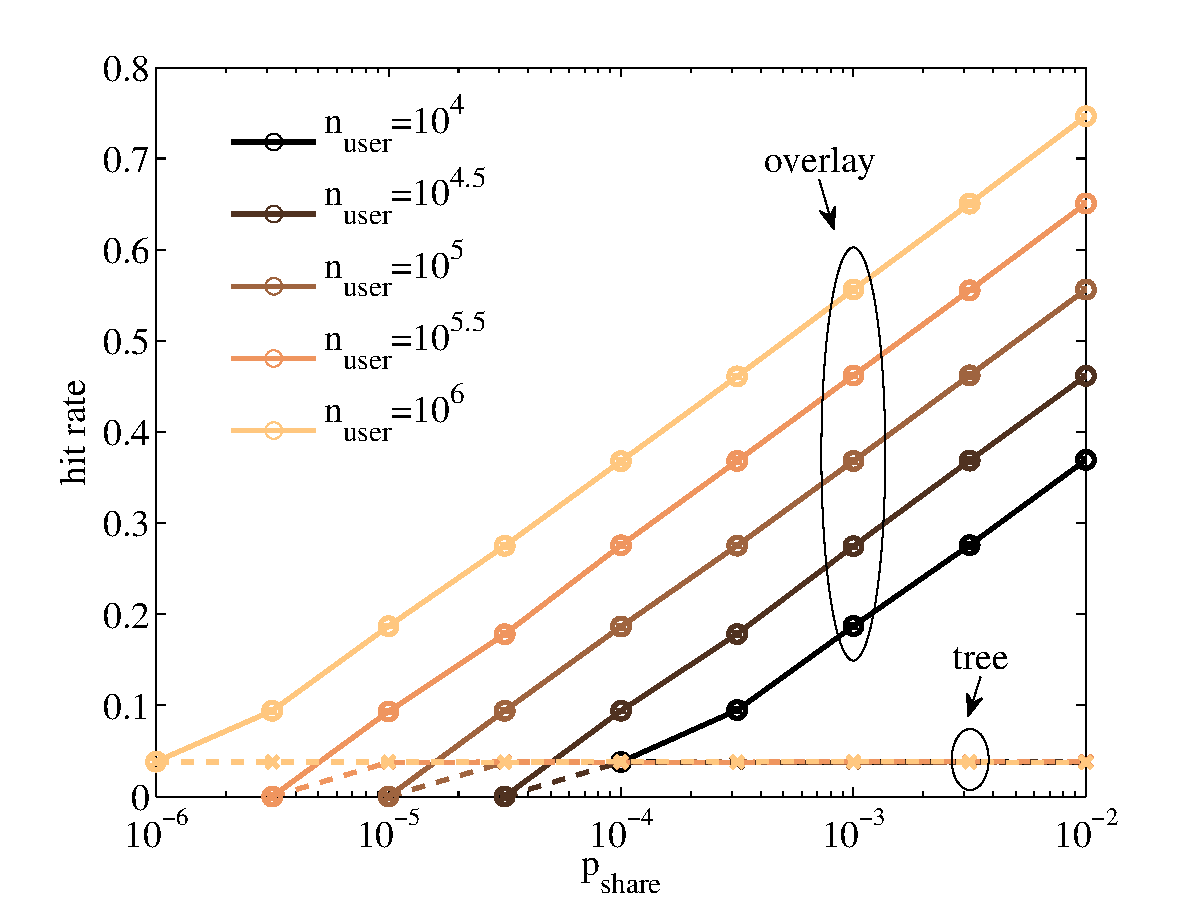
\includegraphics[width=\textwidth]{hierarchical/simulative/figures/overlay_nuser_hitrate}
\caption{Hit rate of the overlay}
\label{fig:overlay_nuser_hitrate}
\end{subfigure}
\begin{subfigure}[t]{0.32\textwidth}
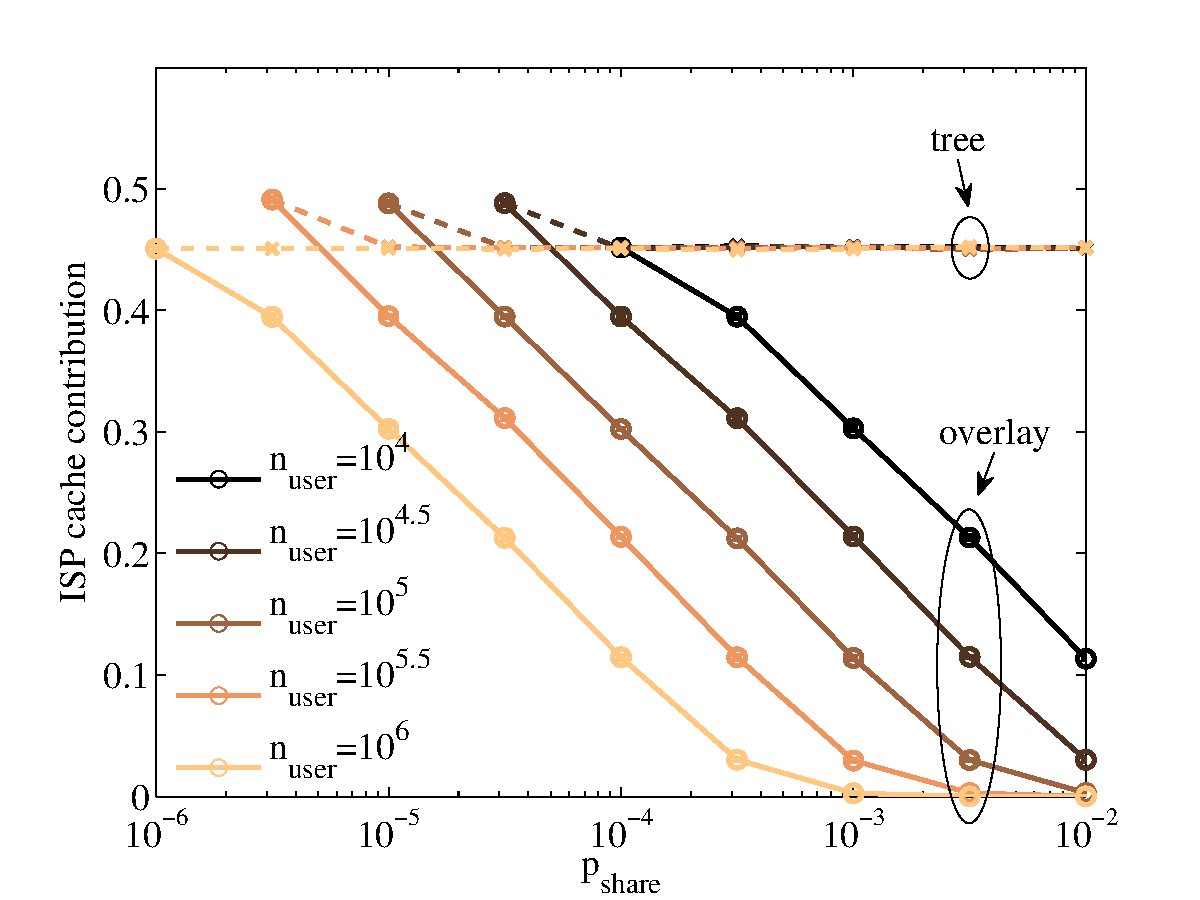
\includegraphics[width=\textwidth]{hierarchical/simulative/figures/overlay_nuser_ISPcontrib}
\caption{ISP cache contribution}
\label{fig:overlay_nuser_ISPcontrib}
\end{subfigure}
\begin{subfigure}[t]{0.32\textwidth}
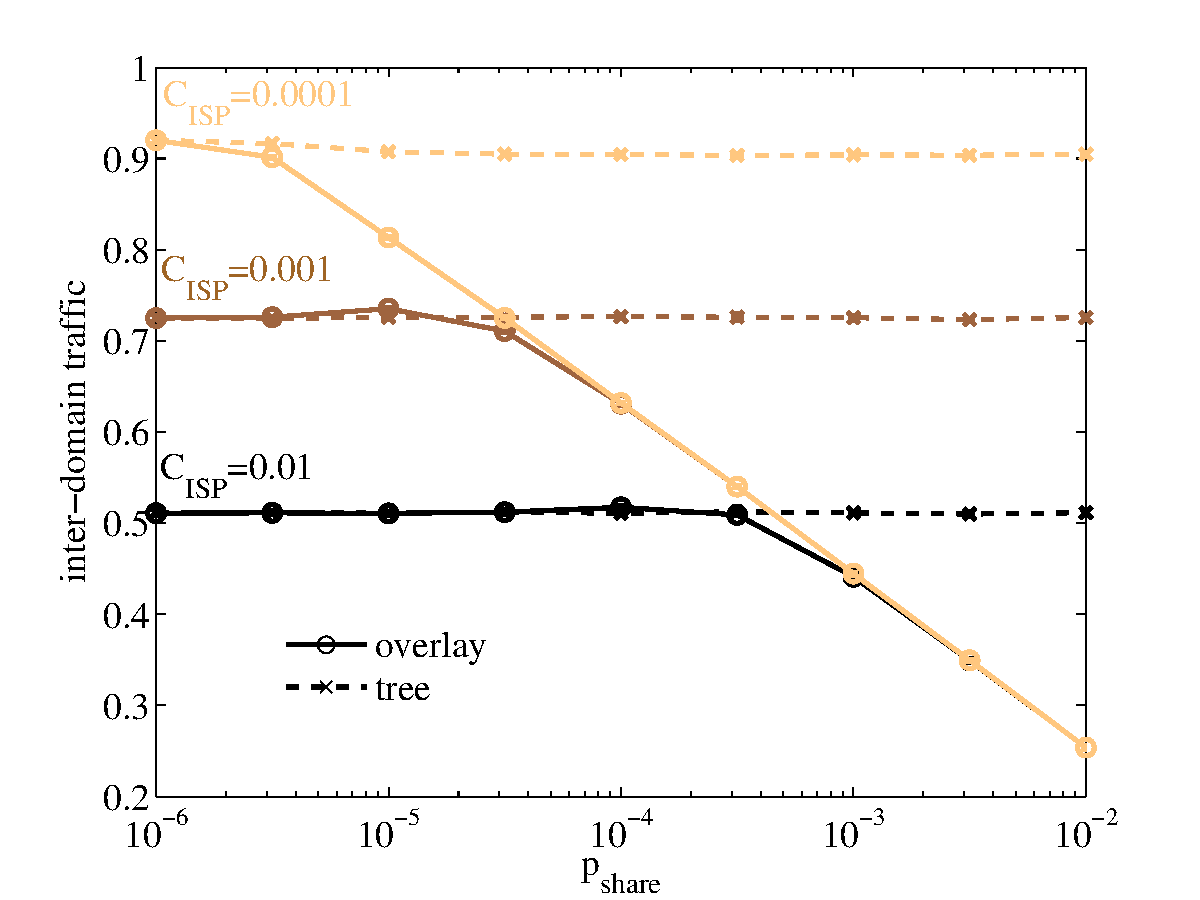
\includegraphics[width=\textwidth]{hierarchical/simulative/figures/overlay_interdomain}
\caption{Inter-domain traffic}
\label{fig:overlay_interdomain}
\end{subfigure}
\caption{Overlay and ISP cache contribution and inter-domain traffic dependent on home router sharing probability.}
\end{figure*}

As the goal of this evaluation is to assess the potential of the overlay and to identify success scenarios, the simulation model assumes that the upload rate of caches is unlimited. However, in practice the upload rate limits the number of requests that can be served by a cache, especially for smaller devices like HRs. The evaluation uses a static and global popularity distribution. In practice the item request process is dynamic and dependent on personal and regional preferences.
The simulation uses a catalog size of $N=10^6$. The results obtained show the average of ten simulation runs with $10^6$ requests and their respective 95\% confidence intervals.
%The hierarchic caching strategy is leave-copy-down, which means that the video is cached in a certain tier only if it is already available in a higher tier.
%In the following we evaluate the performance of the tiered caching architecture. By studying the impact of the home router sharing probability, we identify the amount of home routers, which needs to be shared so that such a mechanism pays off for ISPs. We vary the ISP cache capacity and the Zipf exponent \alpha to investigate to what extent the load on ISP caches can be reduced and how the system performs under various request patterns. For each configuration 5 simulation runs were conducted to achieve significance. The results show the mean value of the 5 runs with 95\% confidence intervals.

Figure~\ref{fig:overlay_nuser_hitrate} shows the hit rate of the overlay dependent on the sharing probability for a constant ISP cache capacity of $C_{ISP}=0.01$. In the tree case, where each user is assigned to a HR as a tier-3 cache, the hit rate is independent of the sharing probability. The hit rate is limited by the cache capacity of the HR. If HRs are organized in an overlay, their hit rate increases with the sharing probability, since requested content items are looked up in all HRs belonging to the overlay. This shows that an overlay highly increases the performance of a caching system with a high number of small caches. Hence, the overlay highly benefits providers and end-users. The hit rate increases with the size of AS $n_{user}$, because a higher total cache capacity is available.

%\begin{figure}[tb]
%\centering
%\includegraphics[width=75mm]{overlay_ISPhitrate}
%\caption{ISP cache hit rate dependent on sharing probability.}
%\label{fig:overlay_ISPhitrate}
%\end{figure}

%Figure~\ref{fig:overlay_ISPhitrate} shows the ISP cache hit rate dependent on the home router sharing probability. The ISP cache hit rate decreases in the overlay case, since popular items are served by the overlay. The ISP cache is only requested for unpopular items which are less likely to be hit. Without overlay the ISP cache gets more efficient with increasing sharing probability, since the branching factor of the tree increases.

%\begin{figure}[tb]
%\centering
%\includegraphics[width=75mm]{overlay_ISPcontrib}
%\caption{ISP cache contribution dependent on sharing probability.}
%\label{fig:overlay_ISPcontrib}
%\end{figure}

Figure~\ref{fig:overlay_nuser_ISPcontrib} shows the ISP cache contribution dependent on the sharing probability for a constant ISP cache capacity of $C_{ISP}=0.01$. In a tree structure the sharing probability has no significant impact on the ISP cache contribution. This depends on the fact that the hit rate of tier-3 caches is low and independent of the sharing probability. All remaining requests are forwarded to the ISP cache and in case of a hit the ISP cache contributes. If the HRs are organized in an overlay, the ISP cache contribution decreases because more requests can be served from the overlay. In this case the ISP cache also gets less efficient because it is only requested for rare items that are not cached in the overlay.
For large ASes with a high number of end-users the ISP cache contribution approaches zero, if at least every thousandth user shares its HR. In this case the ISP cache can be shut down, which saves operating costs and energy. This shows that especially large ASes can benefit from an overlay.

%\begin{figure}[tb]
%\centering
%\includegraphics[width=75mm]{overlay_local}
%\caption{Share of requests served locally dependent on sharing probability.}
%\label{fig:overlay_ISPcontrib}
%\end{figure}

Figure~\ref{fig:overlay_interdomain} shows the inter-domain traffic dependent on the sharing probability for an AS with $n_{user}=10^6$ end-users. If no overlay is present the sharing probability has close to no impact on the amount of requests served locally. In this case the inter-domain traffic can only be reduced by increasing the ISP cache capacity. In the overlay case the number of requests served locally increases with the sharing probability, which decreases the inter-domain traffic. Dependent on the ISP cache capacity a higher fraction of shared HRs is necessary to reduce inter-domain traffic.

\subsubsection{Inter-Domain Traffic}

The overlay is not only used to access content from HRs in the same AS, but also from HRs in neighboring ASes. If the neighboring AS is a peering or customer ISP, no transit costs are incurred.
To assess the inter-domain traffic saved, an AS topology is added to the simulation. The AS relationship dataset provided by caida.org\cite{caida2015} of January 2015 is used and it specifies peering and customer-to-provider links of each AS. The data set consists of 46,172 ASes and 177,000 links.
To be able to process the simulation the topology is limited to RIPE NCC EU ASes. The remaining subset still consists of 31,256 ASes and 77,382 links.
The number of users per AS is determined by evaluating the Internet Census Dataset\cite{carna2013}, which provides a scan on active IP addresses in the Internet. Assuming that the number of users in an AS is proportional to the number of active IP addresses and the probability of a user being in an AS is set accordingly.
To save costly inter-domain traffic and to mitigate load on ISP caches, the following resource selection policy is applied:

If an item is not found on enabled HRs in the same AS, it is requested from other resources in the order:
%(1) HRs in peering ISP ASes, (2) HRs in customer ISP ASes, (3) ISP cache in local AS, (4) ISP cache in peering ISP ASes, (5) ISP cache in customer ISP ASes, and (6) content provider.
%\vspace{2mm}
\begin{enumerate}
	\itemsep0em
	\item HRs in peering ISP ASes
	\item HRs in customer ISP ASes
	\item ISP cache in local AS
	\item ISP cache in peering ISP ASes
	\item ISP cache in customer ISP ASes
	\item content provider
\end{enumerate}

\begin{figure*}[ht!]
\centering
\begin{subfigure}[t]{0.32\textwidth}
\includegraphics[width=\textwidth]{hierarchical/simulative/figures/RBHlocal}
\caption{Share of requests served locally}
\label{fig:RBHlocal}
\end{subfigure}
\begin{subfigure}[t]{0.32\textwidth}
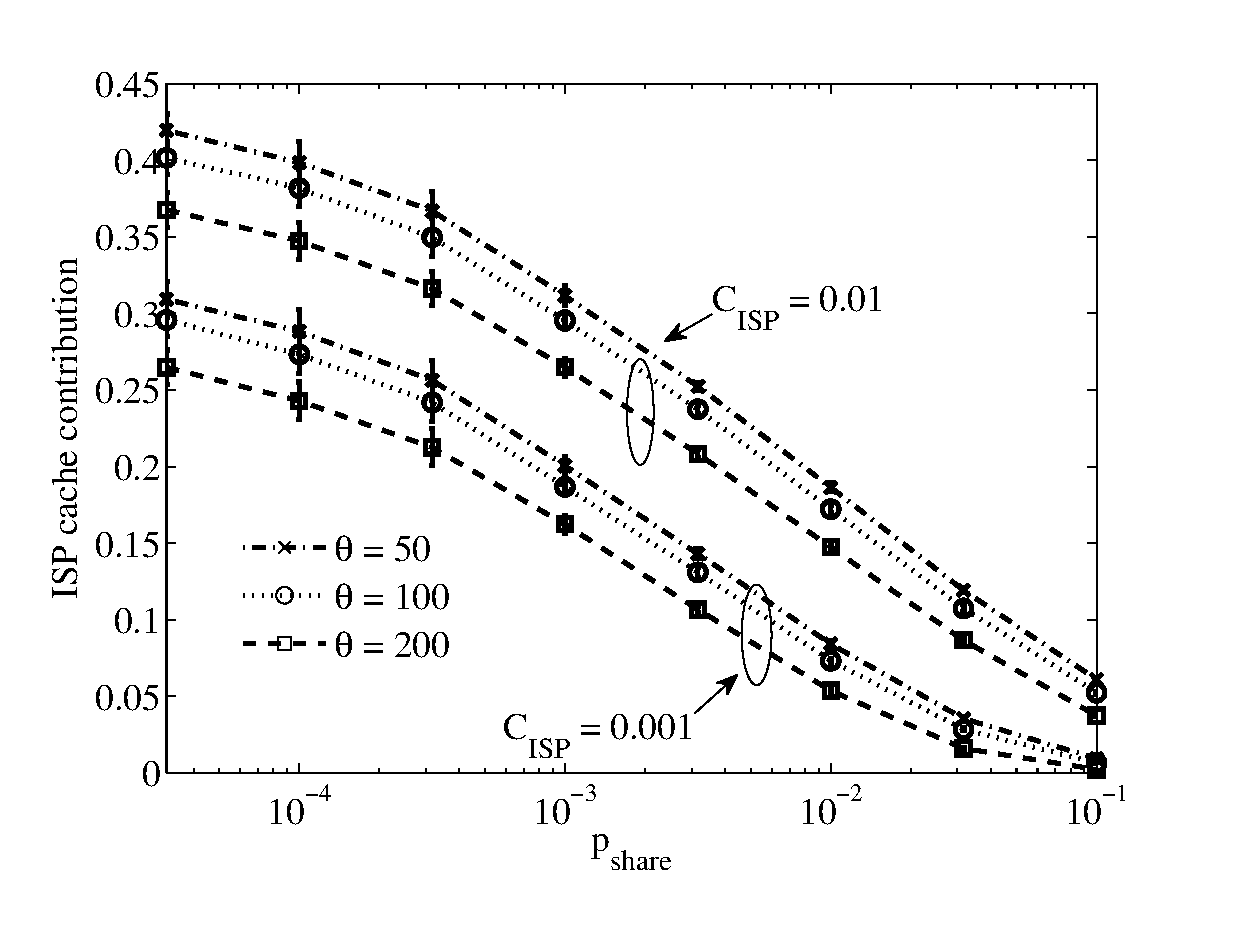
\includegraphics[width=\textwidth]{hierarchical/simulative/figures/ISPcontrib}
\caption{ISP cache contribution}
\label{fig:ISPcontrib}
\end{subfigure}
\begin{subfigure}[t]{0.32\textwidth}
\includegraphics[width=\textwidth]{hierarchical/simulative/figures/RBHall}
\caption{Share of requests served per domain}
\label{fig:RBHall}
\end{subfigure}
\caption{Share of requests served locally and ISP cache contribution dependent on sharing probability and share of requests served per domain.}
\end{figure*}

A policy designed to prioritize ISP caches to remote HRs did not have a significant impact on traffic savings.
%The capacity of ISP caches $C_{ISP}=\{0.001,0.01\}$ is relative to the catalogue size.
The threshold $\theta$ specifies the minimum number of users an AS must have to host an ISP cache. If $\theta=\infty$ no AS hosts an ISP cache and content delivery is solely supported by HRs.
To investigate the performance of our approach, the impact of the HR sharing probability $p_\text{share}$ on the inter-domain traffic and on the ISP cache contribution is studied. The share of traffic within the local AS, peering and customer-to-provider links is evaluated.
For the generation of content item requests a Zipf popularity distribution with slope $\alpha=0.99$ was applied.

%\begin{figure}[tb]
%\centering
%\includegraphics[width=75mm]{RBHlocal}
%\caption{Share of requests served locally dependent on sharing probability.}
%\label{fig:RBHlocal}
%\end{figure}

Figure~\ref{fig:RBHlocal} shows the share of requests served locally dependent on the HR sharing probability. More than 20\% of requests can be served locally, if the ISP cache can store 1\% of the catalog size. With an increasing threshold $\theta$ the number of ASes hosting an ISP cache decreases and, thus, the share of requests being served locally. If the number of shared HRs increases, more traffic can be kept locally. This effect is stronger for a lower ISP cache capacity. In case of $\theta=\infty$ where no ISP caches are available, the sharing probability has the strongest impact on inter-domain traffic. For a high sharing probability the ISP cache size has only little impact on the inter-domain traffic.

Figure~\ref{fig:ISPcontrib} shows the ISP cache contribution dependent on the HR sharing probability. The number of requests an ISP cache can serve increases with its capacity. As for the inter-domain traffic, the sharing probability has a high impact on the ISP cache contribution. For high sharing probabilities the ISP cache contribution approaches zero. This means that ISP caches can be shut down, if a sufficient amount of users would share their HRs.
For a lower threshold $\theta$ more ISP caches are deployed and the ISP cache contribution increases.

%\begin{figure}[tb]
%\centering
%\includegraphics[width=75mm]{RBHall}
%\caption{Share of requests served per domain.}
%\label{fig:RBHall}
%\end{figure}

To study the requests served per domain, the HR sharing probability is set to 1\% and the threshold $\theta$ to 100 users.
Figure \ref{fig:RBHall} shows the share of requests served per domain. Almost none of these requests can be served by the personal HR. This might depend on the fact that items are requested according to a global popularity distribution.
If personal interests are considered in the demand model, higher hit rates and contributions from personal caches are expected. Dependent on the ISP cache capacity, 20 to 25\% of requests can be served locally and 15 to 20\% from neighboring ASes. Still about 2 out of 3 requests are served by the content provider. This depends on the fact that with Zipf slope of $\alpha = 0.99$ content item requests are highly heterogeneous. In practice, temporal and social dynamics of users' interests will lead to temporal and local correlations in requests, which improve the performance of local and personal caches.

%\input{aslevel/census/potential/potential}
